%%%%%%%%%%%%%%%%%%%%%%%%%%%%%%%%%%%%%%%%%%%%%%%%%%%%%%%%%%%%%%%%%%%%%%%
%%%
%%%    【非公式】東京理科大学大学院 創域理工学研究科 機械航空宇宙工学専攻
%%%                         修士論文要旨 テンプレート
%%%
%%%                                  v1.2.0 Yuki MATSUKAWA 21 Dec. 2022
%%%                                  v2.0.0 Yuki MATSUKAWA 25 Dec. 2023
%%%
%%%%%%%%%%%%%%%%%%%%%%%%%%%%%%%%%%%%%%%%%%%%%%%%%%%%%%%%%%%%%%%%%%%%%%%
\documentclass[a4paper,fleqn,dvipdfmx,11pt]{jreport}

%%% abstract style %%%
\usepackage{master_settings}
\usepackage{epsf,color}
\usepackage{float}
\usepackage{subfigure}
\usepackage{rotating}
\usepackage{lscape}
\usepackage{bm}
\usepackage{multirow}
\usepackage{multicol}

% ページ番号を付けない
\pagestyle{empty}

\begin{document}

% 一行あたり文字数の指定
\mojiparline{35}
% 1ページあたり行数の指定
\linesparpage{30}

\begin{center}
\fontsize{12pt}{20pt}\selectfont
% 修士論文題目
ここには修士論文のタイトルを入れます.\\ 一文字でも間違えたら受理されません.
% 修士論文題目
\end{center}

\vskip\baselineskip
\noindent
% 姓と名の間に「全角」スペース忘れずに %
\begin{flushright}
    \begin{tabular}{r @{\hspace{30pt}} r @{\hspace{0pt}\vspace{9pt}}}
        機械航空宇宙工学専攻 & 姓姓姓 名名 \\
        指導教員 & 姓姓 名名
    \end{tabular}
\end{flushright}

\vskip\baselineskip
%%% ここから書き始める %%%
アブストラクトアブストラクトアブストラクトアブストラクトアブストラクトアブストラクトアブストラクトアブストラクトアブストラクト
アブストラクトアブストラクトアブストラクトアブストラクトアブストラクトアブストラクトアブストラクトアブストラクトアブストラクト
アブストラクトアブストラクトアブストラクトアブストラクトアブストラクトアブストラクトアブストラクトアブストラクトアブストラクト
アブストラクトアブストラクトアブストラクトアブストラクトアブストラクトアブストラクトアブストラクトアブストラクトアブストラクト
アブストラクトアブストラクトアブストラクトアブストラクトアブストラクトアブストラクトアブストラクトアブストラクトアブストラクト
アブストラクトアブストラクトアブストラクトアブストラクトアブストラクトアブストラクトアブストラクトアブストラクトアブストラクト
アブストラクトアブストラクトアブストラクトアブストラクトアブストラクトアブストラクトアブストラクトアブストラクトアブストラクト.

アブストラクトアブストラクトアブストラクトアブストラクトアブストラクトアブストラクトアブストラクトアブストラクトアブストラクト
アブストラクトアブストラクトアブストラクトアブストラクトアブストラクトアブストラクトアブストラクトアブストラクトアブストラクト
アブストラクトアブストラクトアブストラクトアブストラクトアブストラクトアブストラクトアブストラクトアブストラクトアブストラクト
アブストラクトアブストラクトアブストラクトアブストラクトアブストラクトアブストラクトアブストラクトアブストラクトアブストラクト
アブストラクトアブストラクトアブストラクトアブストラクトアブストラクトアブストラクトアブストラクトアブストラクトアブストラクト
アブストラクトアブストラクトアブストラクトアブストラクトアブストラクトアブストラクトアブストラクトアブストラクトアブストラクト
アブストラクトアブストラクトアブストラクトアブストラクトアブストラクトアブストラクトアブストラクトアブストラクトアブストラクト.

図~\ref{fig:abst1}は虎,図~\ref{fig:abst2}も虎.
アブストラクトアブストラクトアブストラクトアブストラクトアブストラクトアブストラクトアブストラクトアブストラクトアブストラクト
アブストラクトアブストラクトアブストラクトアブストラクトアブストラクトアブストラクトアブストラクトアブストラクトアブストラクト
アブストラクトアブストラクトアブストラクトアブストラクトアブストラクトアブストラクトアブストラクトアブストラクトアブストラクト
アブストラクトアブストラクトアブストラクトアブストラクトアブストラクトアブストラクトアブストラクトアブストラクトアブストラクト
アブストラクトアブストラクトアブストラクトアブストラクトアブストラクトアブストラクトアブストラクトアブストラクトアブストラクト
アブストラクトアブストラクトアブストラクトアブストラクトアブストラクトアブストラクトアブストラクトアブストラクトアブストラクト
アブストラクトアブストラクトアブストラクトアブストラクトアブストラクトアブストラクトアブストラクトアブストラクトアブストラクト
アブストラクトアブストラクトアブストラクトアブストラクトアブストラクトアブストラクトアブストラクトアブストラクトアブストラクト
アブストラクトアブストラクトアブストラクトアブストラクトアブストラクトアブストラクトアブストラクトアブストラクトアブストラクト
アブストラクトアブストラクトアブストラクトアブストラクトアブストラクトアブストラクトアブストラクトアブストラクトアブストラクト.

\begin{multicols}{2}
   	\begin{figure}[H]
        \centering
   		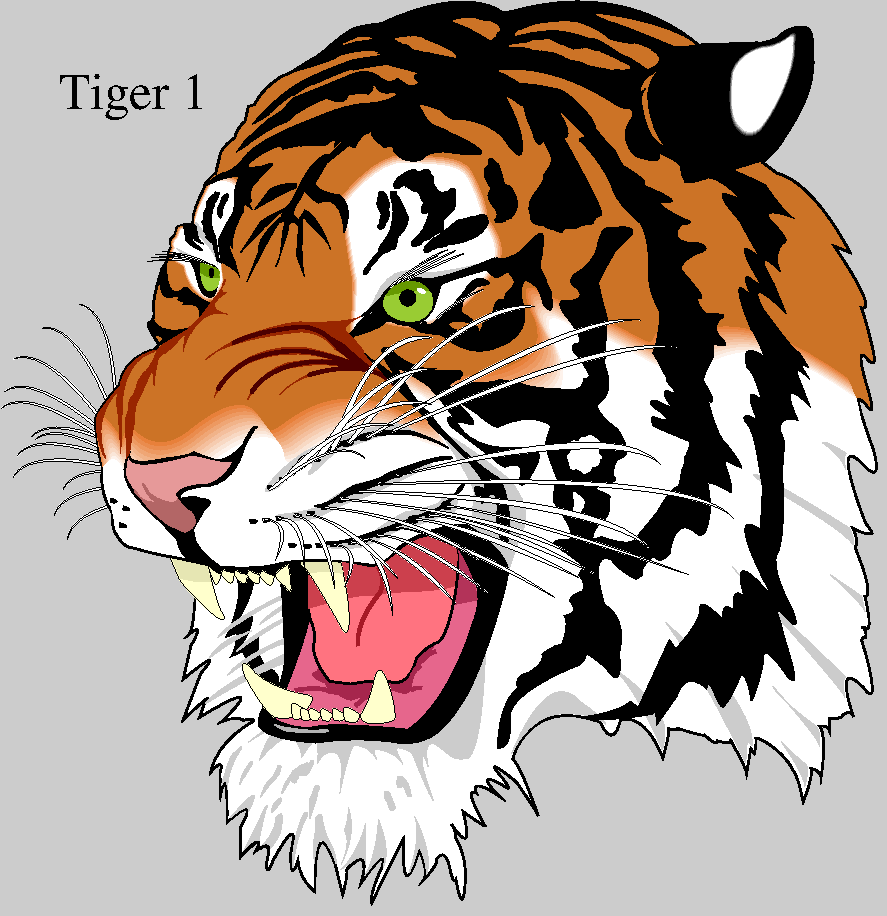
\includegraphics[width=0.6\columnwidth]{tiger_1.pdf}
   		\caption{Tiger 1.}
   		\label{fig:abst1}
   	\end{figure}

   	\begin{figure}[H]
        \centering
   		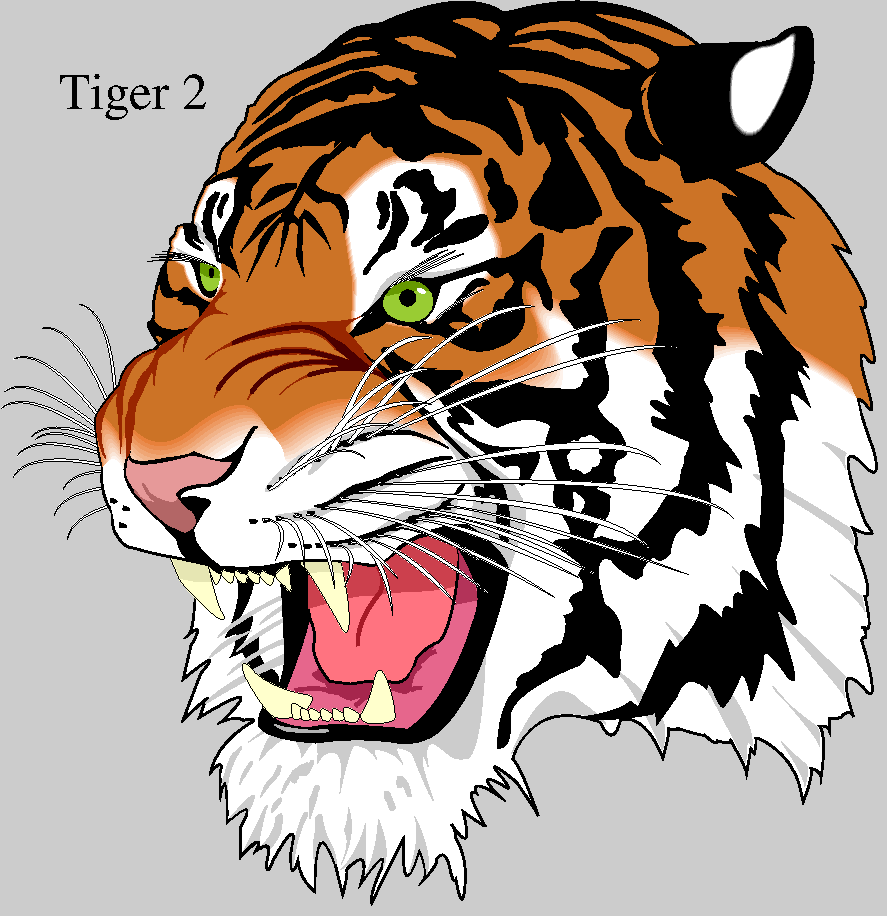
\includegraphics[width=0.6\columnwidth]{tiger_2.pdf}
   		\caption{Tiger 2.}
   		\label{fig:abst2}
   	\end{figure}
\end{multicols}

%%% ここまで %%%

\end{document}
